\documentclass{article}
\usepackage{amsmath}
\usepackage{amsfonts}
\usepackage{pgfplots}

% Make equation numbers depend on the section they belong to
%\numberwithin{equation}{section}
% Make equation numbers depend on the SUBsection they belong to
\numberwithin{equation}{subsection}

\begin{document}

\section{Activation Functions}\label{sec:actfunc}

%%%%%%%%%%%%%%%%%%%%%%%%%%%%%%%%%%%%%%%%%%
%%%%%%%%%%%% SECTION: LINEAR %%%%%%%%%%%%%
%%%%%%%%%%%%%%%%%%%%%%%%%%%%%%%%%%%%%%%%%%
\subsection{Linear}~\label{sec:lin}
\begin{equation}~\label{eq:lin}
  \hat{y} = mx + b
\end{equation}

The functional form of equation~\ref{eq:lin} is shown by figure~\ref{fig:lin}.
\begin{figure}[h!]
  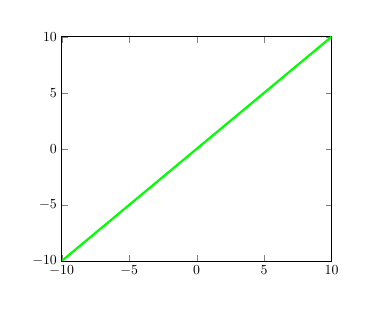
\begin{tikzpicture}[scale=.5]
    \begin{axis}[xmin=-10,xmax=10,ymin=-10,ymax=10]
      \addplot[green,ultra thick,domain=-10:10] {x};
    \end{axis}
  \end{tikzpicture}
  \caption{\small{\textit Linear.}~\label{fig:lin}}
 \end{figure}

%%%%%%%%%%%%%%%%%%%%%%%%%%%%%%%%%%%%%%%%%%
%%%%%%%%%%%% SECTION: RELU %%%%%%%%%%%%%%%
%%%%%%%%%%%%%%%%%%%%%%%%%%%%%%%%%%%%%%%%%%
%\vfill\eject
\subsection{ReLU}\label{sec:relu}
Rectified Linear Unit (ReLU) is defined by:  

\begin{equation}
\hat{y}=\begin{cases}
          \quad wx+b \quad &\text{if}~wx+b > 0 \\
          \quad 0 \quad &\text{Otherwise.}\\
     \end{cases}
  \end{equation}
From this we see that negative outputs are set to $0$.
Using ReLU in hidden layers adds efficient non-linearity.

%\begin{figure}[H]
  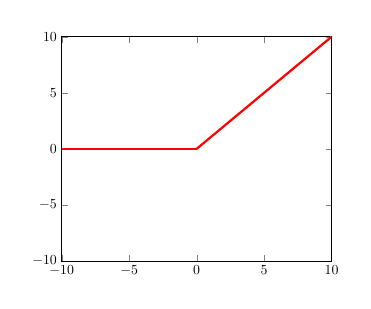
\begin{tikzpicture}[scale=.5]
    \begin{axis}[
      xmin = -10, xmax = 10,
      ymin = -10, ymax = 10]
      \addplot[
        red,
        ultra thick,
        domain = -10:0,
      ] {0};
      \addplot[
        red,
        ultra thick,
        domain = 0:10,
      ] {x};
    \end{axis}
  \end{tikzpicture}
%\end{figure}

%%%%%%%%%%%%%%%%%%%%%%%%%%%%%%%%%%%%%%%%%%
%%%%%%%%%%%% SECTION: SIGMOID %%%%%%%%%%%%
%%%%%%%%%%%%%%%%%%%%%%%%%%%%%%%%%%%%%%%%%%
\vfill\eject
\subsection{Sigmoid}\label{sec:sigmoid}

Using a Sigmoid function at the end/output generates a 
probability for each digit (in the case of mnist data).  Using 
the $softmax$ function causes all sigmoid probabilities to be 
re-weighted, such that the sum to unity.

\begin{equation}
  \hat{y} = \frac{1}{1 + e^{-(wx+b)}}
\end{equation}


%\resizebox{1}{1}

%\section{}


\end{document}